\documentclass[11pt, oneside]{article}
\usepackage[margin=.9in]{geometry}
\usepackage{pgfplots}
\pgfplotsset{compat=default}
\newcommand{\cuckoo}{{\rm cuckoo}}
\newcommand{\sha}{{\rm SHA256}}
\usepackage{hyperref}
\title{Cuckoo Cycle \protect\\ a memory-hard proof-of-work system}
\author{John Tromp}
\begin{document}
\maketitle
\section{Introduction}
A ``proof of work'' (PoW) system allows a verifier to check---with
negligible effort---that a prover has expended a large amount of computational effort.
Originally introduced as a spam fighting measure, 
where the effort is the price paid by an email sender for demanding the recipient's attention,
they now form one of the cornerstones of crypto-currencies.

Bitcoin\cite{nakamoto2009bitcoin} uses hashcash\cite{back2002} as proof of work for
new blocks of transactions, which requires finding a nonce value such that
twofold application of the cryptographic hash function SHA256
to this nonce (and the rest of the block header) results in a number with many
leading 0s.  The bitcoin protocol dynamically adjust this ``difficulty'' number
so as to maintain a 10-minute average block interval. Starting out at 32 leading zeroes in 2009,
the number has steadily climbed and is currently at 63, representing
an incredible $2^{63}/10$ double-hashes per minute. This exponential growth of hashing power
is enabled by the highly-parallellizable nature of the hashcash proof of work.
which saw desktop cpus out-performed by graphics-cards,
these in turn by programmable gate arrays, and finally by custom designed chips (ASICs).

Downsides of this development include high investment costs, rapid obsolesence, centralization
of mining power, and ``waste'' of energy.
This has led people to look for alternative proofs of work that lack parallelizability,
aiming to keep commodity hardware competitive.

Litecoin replaces the sha256 hash function in hashcash by a single round, 128KB version of the
{\em scrypt} key derivation function. Technically, this is no longer a proof of work system, as
verification takes a nontrivial amount of computation. Even so, GPUs are a least an order
of magnitude faster than CPUs for Litecoin mining, and ASICs are coming on to the market in 2014.

Primecoin~\cite{king2013} is an interesting design based on finding long Cunningham chains
of prime numbers, using a two-step process of filtering candidates by {\em sieving}, and applying
pseudo-primality tests to remaining candidates. The most efficient implementations are still CPU based.
A downside to primecoin is that its use of memory is not constrained much.

\section{Memory latency; the great equalizer}
To level the mining playing field, a proof of work system should not merely be memory bound rather
than CPU bound, it should have the following additional properties:
\begin{description}
\item[scalable] The amount of memory needed should be a parameter that can scale arbitrarily.
\item[linear] The number of memory accesses should be linear in the amount---on average,
each memory cell is accessed a constant number of time
\item[tmto-hard] It should not allow any time-memory trade-off---using only half as much memory should incur
several orders of magnitude slowdown.
\item[no-locality] The pattern of memory accesses should be sufficiently random as to make caches useless.
\item[cpu-easy] the total running time should be dominated by waiting for memory accesses
\item[simple] The algorithm should be sufficiently simple that one can be convinced of its optimality.
\end{description}
Combined, these properties ensure that the proof of work system is almost entirely constrained by main
memory latency and scales appropriately for any application.

We introduce the first proof of work system satisfying these properties.
Amazingly, it amounts to little more than enumerating nonces and storing them
in a hashtable. All hashtables break down when trying to store more items than
it was designed to handle. For one particular hash table design, this very break down
is of a special form that can be turned into a concise and quickly verifiable proof.
Enter the cuckoo hash table.

\section{Cuckoo hashing}
Introduced by Rasmus Pagh and Flemming Friche Rodler in
2001\cite{Pagh01cuckoohashing}, a cuckoo hash table consists of two same sized
hash tables with different hash functions,
providing two possible locations for each key (and constant lookup time).
Upon insertion of a new key, if both locations are already taken,
then one is kicked out and inserted in its alternate location, possibly
displacing yet another key, repeating the process until either a vacant
location is found, or some maximum number of iterations,
is reached. The latter can only happen once cycles have formed in the {\em
Cuckoo graph}.  This is a bipartite graph with a node for each location and an
edge for every key,
connecting the two locations it can reside at. This naturally suggests a proof
of work problem, which we now formally define.

\section{The proof of work function}
Fix three parameters $L \leq E \leq N$ in the range $\{4,...,2^{32}\}$, which
denote the cycle length, number of edges (also easyness, opposite of difficulty),
and the number of nodes, resprectively. $L$ and $N$ must be even.
Function $\cuckoo$ maps any binary string $h$ (the header) to a bipartite graph
$G = (V_0 \cup V_1, E)$, where $V_0$ is the set of integers modulo $N_0=N/2+1$,
$V_1$ is the set of integers modulo $N_1=N/2-1$, and $E$ has an edge between
$\sha(h\;n) \bmod N_0$ in $V_0$ and $\sha(h\;n) \bmod N_1$ in $V_1$ for every
nonce $0 \leq n < E$. A proof for $G$ is a subset of $L$ nonces whose
corresponding edges form an $L$-cycle in $G$.

\section{Cycle formation}
A set of stored keys gives rise to a {\em directed} cuckoo graph, where each
stored key is a directed edge from the location where it resides to its
alternate location. The outdegree of every node in this
graph is either 0 or 1, When there are no cycles yet, the graph is a {\em
forest}, a disjoint union of trees. In each tree, all edges are directed,
directly, or indirectly, to its root,
the only node in the tree with outdegree 0. Addition of a new key causes a
cycle if and only if its two locations are in the same tree, testable
by following the path each locations to its root.
In case of equal roots, we can compute the length of the resulting cycle as
1 plus the sum of the path-lengths to the node where the two paths first join.
If the cycle length is not $L$, we keep the graph acyclic by not storing the new key.
There is some probability of overlooking other $L$-cycles
that uses that key, but in the important low easyness case of having few cycles
in the cuckoo graph to begin with, it does not significantly affect
the rate of solution finding.

\section{Implementation and performance}
The C-program listed in the Appendix is also available online at
\url{https://github.com/tromp/cuckoo} together with a Makefile,
proof verifier and this paper. `make test' tests everything.
The main program uses 31 bits per node to represent the
directed cuckoo graph, reserving the most significant bit
for marking edges on a cycle, to simplify recovery of the proof nonces.
On my 3.2GHz Intel Core i5, in case no solution is found, size $2^{20}$ takes 4MB and 0.25s, size
$2^{25}$ takes 128MB and 10s, and size $2^{30}$ takes 4GB and 400s, a significant fraction of which
is spend pointer chasing.
Figure~\ref{solprob} shows the probability of finding a 42-cycle as empirically
determined from 10000 runs at size $1 \cdot 2^{20}$.  Figure~\ref{readswrites} shows that on average,
for each edge, 3.3 reads and 1.75 writes to main memory take place.
For optimal performance, the implementation should be multi-threaded, with one thread enumerating
edges, and the other accessing memory.

\section{Memory-hardness}
I conjecture that this problem doesn't allow for a time-memory trade-off. If
one were to store only a fraction $p$ of $V_0$ and $V_1$, then one would have
to reject a fraction $p^2$ of generated edges, drastically reducing the odds of
finding cycles for $p<1/\sqrt{2}$ (the reduction being exponential in cycle length).
There is one obvious trade-off in the other direction. By doubling the memory
used, nonces can be stored alongside the directed edges, which would save the
effort of recovering them in the current slow manner. The speedup falls far
short of a factor 2 though, so a better use of that memory would be to run
another copy in parallel.

\section{Choice of cycle length}
Extremely small cycle lengths risk the feasability of alternative datastructures that
are more memory-efficient. For example, for $L=2$ the problem reduces to finding a birthday collision,
for which a Bloom filter would be very effective, as would Rainbow tables.
It seems however that the Cuckoo representation might be optimal even for $L=4$.
Such small values still harm the TMTO resistance though as mentioned in the previous paragraph.
In order to keep proof size manageable, the cycle length should not be too large either.
We consider 24-64 to be a healthy range. The chosen value of 42 is close to the middle of the range.

\section{Scaling memory beyond 16-32GB}
While the current algorithm can accomodate up to $N=2^{33}-2$ nodes by a simple change
in implementation, a different idea is needed to scale beyond that.
To that end, we propose to use $K$-partite graphs with edges only between partition $k$ and partition $(k+1) \bmod K$,
where $k$ is fed into the hash function along with the header and nonce. With each partition consisting of at most
$2^31-1$ nodes, the most significant bit is then available to distinguish edges to the two neighbouring partitions.

\bibliographystyle{plain}
\bibliography{cuckoo}

\section{Appendix A: cuckoo.c Source Code}
\footnotesize
\begin{verbatim}
// Cuckoo Cycle, a memory-hard proof-of-work
// Copyright (c) 2013-2014 John Tromp

#include "cuckoo.h"
// algorithm parameters
#define MAXPATHLEN 65536

// used to simplify nonce recovery
#define CYCLE 0x80000000
int cuckoo[1+SIZE]; // global; conveniently initialized to zero

int main(int argc, char **argv) {
  // 6 largest sizes 131 928 529 330 729 132 not implemented
  assert(SIZE < (unsigned)CYCLE);
  char *header = argc >= 2 ? argv[1] : "";
  printf("Looking for %d-cycle on cuckoo%d%d(\"%s\") with %d edges\n",
               PROOFSIZE, SIZEMULT, SIZESHIFT, header, EASYNESS);
  int us[MAXPATHLEN], nu, u, vs[MAXPATHLEN], nv, v; 
  for (int nonce = 0; nonce < EASYNESS; nonce++) {
    sha256edge(header, nonce, us, vs);
    if ((u = cuckoo[*us]) == *vs || (v = cuckoo[*vs]) == *us)
      continue; // ignore duplicate edges
    for (nu = 0; u; u = cuckoo[u]) {
      assert(nu < MAXPATHLEN);
      us[++nu] = u;
    }
    for (nv = 0; v; v = cuckoo[v]) {
      assert(nv < MAXPATHLEN);
      vs[++nv] = v;
    }
#ifdef SHOW
    for (int j=1; j<=SIZE; j++)
      if (!cuckoo[j]) printf("%2d:   ",j);
      else            printf("%2d:%02d ",j,cuckoo[j]);
    printf(" %x (%d,%d)\n", nonce,*us,*vs);
#endif
    if (us[nu] == vs[nv]) {
      int min = nu < nv ? nu : nv;
      for (nu -= min, nv -= min; us[nu] != vs[nv]; nu++, nv++) ;
      int len = nu + nv + 1;
      printf("% 4d-cycle found at %d%%\n", len, (int)(nonce*100L/EASYNESS));
      if (len != PROOFSIZE)
        continue;
      while (nu--)
        cuckoo[us[nu]] = CYCLE | us[nu+1];
      while (nv--)
        cuckoo[vs[nv+1]] = CYCLE | vs[nv];
      for (cuckoo[*vs] = CYCLE | *us; len ; nonce--) {
        sha256edge(header, nonce, &u, &v);
        if (cuckoo[u] == (CYCLE|v) || cuckoo[v] == (CYCLE|u))
          printf("%2d %08x (%d,%d)\n", --len, nonce, u, v);
      }
      break;
    }
    while (nu--)
      cuckoo[us[nu+1]] = us[nu];
    cuckoo[*us] = *vs;
  }
  return 0;
}
\end{verbatim}

\section{Appendix B: cuckoo.h Header File}
\footnotesize
\begin{verbatim}
// Cuckoo Cycle, a memory-hard proof-of-work
// Copyright (c) 2013-2014 John Tromp

#include <stdio.h>
#include <stdint.h>
#include <string.h>
#include <assert.h>
#include <openssl/sha.h>

// proof-of-work parameters
#ifndef SIZEMULT 
#define SIZEMULT 1
#endif
#ifndef SIZESHIFT 
#define SIZESHIFT 20
#endif
#ifndef EASYNESS 
#define EASYNESS (SIZE/2)
#endif
#ifndef PROOFSIZE 
#define PROOFSIZE 42
#endif

#define SIZE (SIZEMULT*(1<<SIZESHIFT))
// relatively prime partition sizes
#define PARTU (SIZE/2+1)
#define PARTV (SIZE/2-1)

// generate edge in cuckoo graph from hash(header++nonce)
void sha256edge(char *header, int nonce, int *pu, int *pv) {
  uint32_t hash[8];
  SHA256_CTX sha256;
  SHA256_Init(&sha256);
  SHA256_Update(&sha256, header, strlen(header));
  SHA256_Update(&sha256, &nonce, sizeof(nonce));
  SHA256_Final((unsigned char *)hash, &sha256);
  uint64_t u64 = 0, v64 = 0;
  for (int i = 8; i--; ) {
    u64 = ((u64<<32) + hash[i]) % PARTU;
    v64 = ((v64<<32) + hash[i]) % PARTV;
  }
  *pu = 1 +         (int)u64;
  *pv = 1 + PARTU + (int)v64;
}
\end{verbatim}

\section{Appendix C: plots}

\begin{figure}
\centering
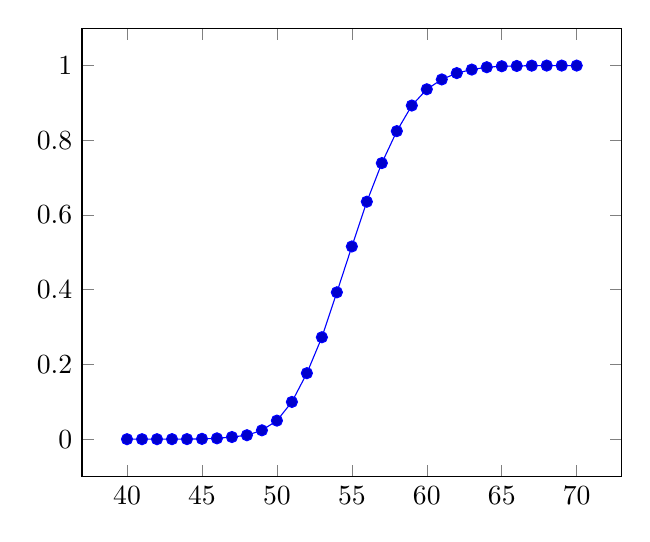
\begin{tikzpicture}
\begin{axis}
\addplot coordinates {
% (1,0) (2,0) (3,0) (4,0) (5,0) (6,0) (7,0) (8,0) (9,0) (10,0)
% (11,0) (12,0) (13,0) (14,0) (15,0) (16,0) (17,0) (18,0) (19,0) (20,0)
% (21,0) (22,0) (23,0) (24,0) (25,0) (26,0) (27,0) (28,0) (29,0) (30,0)
% (31,0) (32,0) (33,0) (34,0) (35,0) (36,0) (37,0) (38,0) (39,0)
(40,0) (41,0) (42,0) (43,0.0001) (44,0.0002) (45,0.0009)
(46,0.0022) (47,0.0058) (48,0.0106) (49,0.0237) (50,0.0497)
(51,0.0997) (52,0.1767) (53,0.2728) (54,0.3931) (55,0.5158)
(56,0.6357) (57,0.739) (58,0.8246) (59,0.8931) (60,0.9366)
(61,0.9629) (62,0.9799) (63,0.9893) (64,0.9956) (65,0.9982)
(66,0.999) (67,0.9998) (68,1) (69,1) (70,1)
% (71,1) (72,1) (73,1) (74,1) (75,1) (76,1) (77,1) (78,1) (79,1) (80,1)
% (81,1) (82,1) (83,1) (84,1) (85,1) (86,1) (87,1) (88,1) (89,1) (90,1)
% (91,1) (92,1) (93,1) (94,1) (95,1) (96,1) (97,1) (98,1) (99,1) (100,1)
};
\end{axis}
\end{tikzpicture}
\caption{Solution probability as function of percentage edges/nodes}
\label{solprob}
\end{figure}

\begin{figure}
\centering
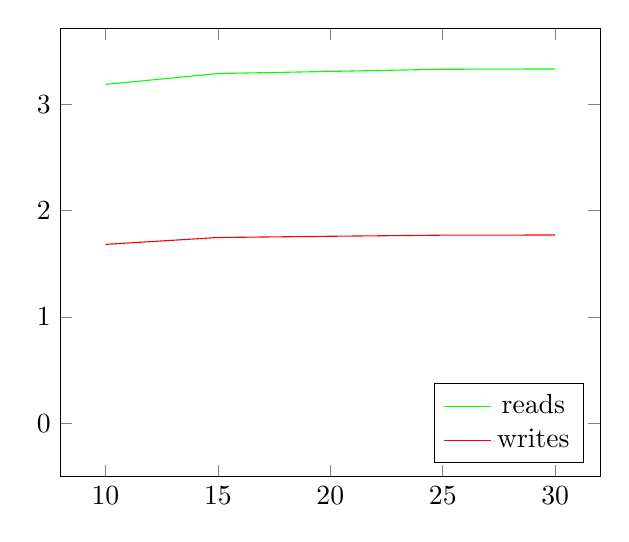
\begin{tikzpicture}
\begin{axis}[ymin=-.5, legend pos=south east]
\addplot[color=green] coordinates { (10,3.1882) (15,3.2904) (20,3.3104) (25,3.3308) (30,3.3333) };
\addlegendentry{reads}
\addplot[color=red]   coordinates { (10,1.6836) (15,1.7482) (20,1.7599) (25,1.7703) (30,1.7717) };
\addlegendentry{writes}
\end{axis}
\end{tikzpicture}
\caption{average memory reads and writes per edge as function of log size}
\label{readswrites}
\end{figure}

\end{document}  
